\documentclass[a4paper, 10pt]{article}

%%%%%%%%%%%%%%%%%%%%%%%%%%%%%%%%%%%%%%%%%%%%%%%%%%%%%%%%%%%%%%%%%%%%%%%%%%%%%%%%%%%%%%%%%%%%%%%%%
%
% Packages
%
% Here you can declare the packages you are going to use in your research paper.
% You can also setup the configuration for some of those packages.
%
\usepackage[utf8]{inputenc}
\usepackage[english]{babel}
\usepackage[style=apa,backend=biber]{biblatex}
\usepackage{hyperref}
\usepackage{graphicx}
\usepackage{csquotes}
\usepackage{amssymb}
\usepackage{amsmath}
\usepackage{xcolor}
\usepackage{braket}
\usepackage{a4wide}
%\usepackage{multirow}            % Expands the content of a cell into multiple rows.
%\usepackage{subcaption}          % Adds a separate \caption for each subfigure.
%\usepackage{multicol}            % Expands the content of a cell into multiple columns.

% Language declaration for the APA referencing style
\DeclareLanguageMapping{english}{english-apa}

% Color setup for the hyperlinks
\hypersetup{
  colorlinks,
  linkcolor={red!90!black},
  citecolor={green!90!black},
  urlcolor={magenta!90!black}
}
%
%%%%%%%%%%%%%%%%%%%%%%%%%%%%%%%%%%%%%%%%%%%%%%%%%%%%%%%%%%%%%%%%%%%%%%%%%%%%%%%%%%%%%%%%%%%%%%%%%


%%%%%%%%%%%%%%%%%%%%%%%%%%%%%%%%%%%%%%%%%%%%%%%%%%%%%%%%%%%%%%%%%%%%%%%%%%%%%%%%%%%%%%%%%%%%%%%%%
%
% Definitions
%
% Here I introduced some definitions for your research paper.
%
\addto{\captionsenglish}{\renewcommand{\abstractname}{Summary}}
%
% The following 4 definitions are required by the toy example.
% You can remove/comment them when creating your own research paper.
%
\newcommand{\Prob}[1]{\mathbf{Pr}\left\{ #1 \right\}}
%
%%%%%%%%%%%%%%%%%%%%%%%%%%%%%%%%%%%%%%%%%%%%%%%%%%%%%%%%%%%%%%%%%%%%%%%%%%%%%%%%%%%%%%%%%%%%%%%%%

%%%%%%%%%%%%%%%%%%%%%%%%%%%%%%%%%%%%%%%%%%%%%%%%%%%%%%%%%%%%%%%%%%%%%%%%%%%%%%%%%%%%%%%%%%%%%%%%%
%
% Bibliography file
%
% This file must follow the bibtex reference format. See the toy example.
%
\bibliography{biblio}
%
%%%%%%%%%%%%%%%%%%%%%%%%%%%%%%%%%%%%%%%%%%%%%%%%%%%%%%%%%%%%%%%%%%%%%%%%%%%%%%%%%%%%%%%%%%%%%%%%%


\begin{document}          % Start of your research paper.


%%%%%%%%%%%%%%%%%%%%%%%%%%%%%%%%%%%%%%%%%%%%%%%%%%%%%%%%%%%%%%%%%%%%%%%%%%%%%%%%%%%%%%%%%%%%%%%%%
%
% Title page
%
% You have to modify this information adapting it to your own research paper. 
%
\title{Quantum Supremacy}
\author{
Student1's name, Student2's name \\
Amsterdam University of Applied Science \\
Amsterdam, The Netherlands \\
\{student1.email, student2.email\}@hva.nl
}
%
%%%%%%%%%%%%%%%%%%%%%%%%%%%%%%%%%%%%%%%%%%%%%%%%%%%%%%%%%%%%%%%%%%%%%%%%%%%%%%%%%%%%%%%%%%%%%%%%%

\maketitle                % Creates the Title page for your research paper.


%%%%%%%%%%%%%%%%%%%%%%%%%%%%%%%%%%%%%%%%%%%%%%%%%%%%%%%%%%%%%%%%%%%%%%%%%%%%%%%%%%%%%%%%%%%%%%%%%
%
% Abstract
%
% Here you have to write down the Abstract/Summary/Samenvatting of your research paper.
%
\begin{abstract}
The promise of quantum computers is that certain computational tasks might be
executed exponentially faster on a ...
\end{abstract}
%
%%%%%%%%%%%%%%%%%%%%%%%%%%%%%%%%%%%%%%%%%%%%%%%%%%%%%%%%%%%%%%%%%%%%%%%%%%%%%%%%%%%%%%%%%%%%%%%%%


%\clearpage                % Forces LaTeX to produce a page break.
%\tableofcontents          % Creates the Table of Content for your research paper.
%\clearpage                % Forces LaTeX to produce a page break.


%%%%%%%%%%%%%%%%%%%%%%%%%%%%%%%%%%%%%%%%%%%%%%%%%%%%%%%%%%%%%%%%%%%%%%%%%%%%%%%%%%%%%%%%%%%%%%%%%
%
% Sections of the paper
%
% Here you have to introduce every LaTeX file that is part of your research paper.
% Use the \input{•} command to do so. Get used to define each differen section in a
% separate .tex file; for instance, my research paper contains 6 sections therefore 
% I have 6 different files.
%
\section{Introduction}
\label{sec:introduction}

The car should have the following features:
\begin{itemize}
    \item The car should have a key that can be inserted and removed. The car should only work when the key is inserted.
    \item The car should have a gearbox with 4 different states: OFF, PARK, DRIVE, and BACK.
    \item The car should have a motor that can be controlled by the gearbox. The motor should be able to rotate clockwise and counterclockwise.
    \item The car should have a display that shows the state of the car.
    \item The car should have turn signals that can be activated by the gearbox.
    \item The car should have a horn that can be activated by a button.
    \item The car should have a brake that can be activated by a button.
\end{itemize}

I had to use several components given to me.

\section{A suitable computational task}
\label{sec:task}
To demonstrate quantum supremacy, we compare our quantum processor against ...

%%%%%%%%%%%%%%%%%%%%%%%%%%%%%%%%%%%%%%%%%%%%%%%%%%%%%%%%%%%%%%%%%%%%%%%%%%%%%%%%%%%%%%%%%%%%%%%%%
%
% This paragraph contains an example of math mode. This is an special and
% powerful mode that allows you to easily create math formulas and scientific
% environments. Use the special characters $ $ to enclose a math mode section.
% If you need it for your research paper, let me know and I will help you out.
%
% It also contains an example of italic format. Use the command \textit{•} to
% produce an italic format.
%
%%%%%%%%%%%%%%%%%%%%%%%%%%%%%%%%%%%%%%%%%%%%%%%%%%%%%%%%%%%%%%%%%%%%%%%%%%%%%%%%%%%%%%%%%%%%%%%%%
For a given circuit, we collect the measured bitstrings $\{x_{i}\}$ and compute
the \textit{linear cross--entropy benchmarking fidelity}, which is the mean of
the simulated probabilities of the bitstrings we measured:

%%%%%%%%%%%%%%%%%%%%%%%%%%%%%%%%%%%%%%%%%%%%%%%%%%%%%%%%%%%%%%%%%%%%%%%%%%%%%%%%%%%%%%%%%%%%%%%%%
%
% The following paragraph contains an example of an equation. Use the environments
% \begin{equation} \begin{split} ... \end{split} \end{equation} to create a numered
% multi-line equation. Each line is limited by the character '\\'. In order to align
% the equation you can use the character '&'.
%
% The equation within a research paper are identified by a number. This is done
% automatically by LaTeX. You have to define a \label{•} for future references.
%
%%%%%%%%%%%%%%%%%%%%%%%%%%%%%%%%%%%%%%%%%%%%%%%%%%%%%%%%%%%%%%%%%%%%%%%%%%%%%%%%%%%%%%%%%%%%%%%%%
\begin{equation}
  \begin{split}
    \mathcal{F}_{\text{XEB}} &= 2^{n} \braket{\Prob{x_{i}}}_{i} - 1, \\
  \end{split}
  \label{eq:fidelity}
\end{equation}

where $n$ is the number of ...

\section{Building a high--fidelity processor}
\label{sec:processor}
%%%%%%%%%%%%%%%%%%%%%%%%%%%%%%%%%%%%%%%%%%%%%%%%%%%%%%%%%%%%%%%%%%%%%%%%%%%%%%%%%%%%%%%%%%%%%%%%%
%
% The following paragraph contains an example of an internal reference. Use the
% command \ref{•} along with the identifier defined with the command \label{•} to create
% a reference to an internal section on your research paper. The label can be defined in
% any of the .tex files that you have included.
%
%%%%%%%%%%%%%%%%%%%%%%%%%%%%%%%%%%%%%%%%%%%%%%%%%%%%%%%%%%%%%%%%%%%%%%%%%%%%%%%%%%%%%%%%%%%%%%%%%
We designed a quantum processor named ``Sycamore'', shown in
Figure~\ref{fig:sycamore_processor}, which consists of a two--dimensional array
of 54 transmon qubits, where each qubit is tunably coupled to four nearest
neighbors, in a rectangular lattice.

%%%%%%%%%%%%%%%%%%%%%%%%%%%%%%%%%%%%%%%%%%%%%%%%%%%%%%%%%%%%%%%%%%%%%%%%%%%%%%%%%%%%%%%%%%%%%%%%%
%
% The following paragraph contains several examples:
%
%   1.- A figure. Use the environment \begin{figure} ... \end{figure} to insert
%       an image.
%
%   2.- Centering in the page. Use the command \centering to center horizontally
%       in the page
%
%   3.- Define the image to insert. Use the command \includegraphics[scale=•]{•}
%       to select the image to be inserted. Change the size of the image with the
%        scale parameter and provide the relative path to the image.
%
%   4.- Create a caption for the image. Use the command \caption{•} to include an 
%       explanatory text of the image. Be as self-contained as possible.
%
%   5.- Math mode. Use the characters $ $ to enclose a math mode section within
%       your text.
%
%   6.- Definition of the label. Use the command \label{•} to be used/referenced in
%       a different section of your research paper.
%
%%%%%%%%%%%%%%%%%%%%%%%%%%%%%%%%%%%%%%%%%%%%%%%%%%%%%%%%%%%%%%%%%%%%%%%%%%%%%%%%%%%%%%%%%%%%%%%%%
\begin{figure}[t]
  \centering
  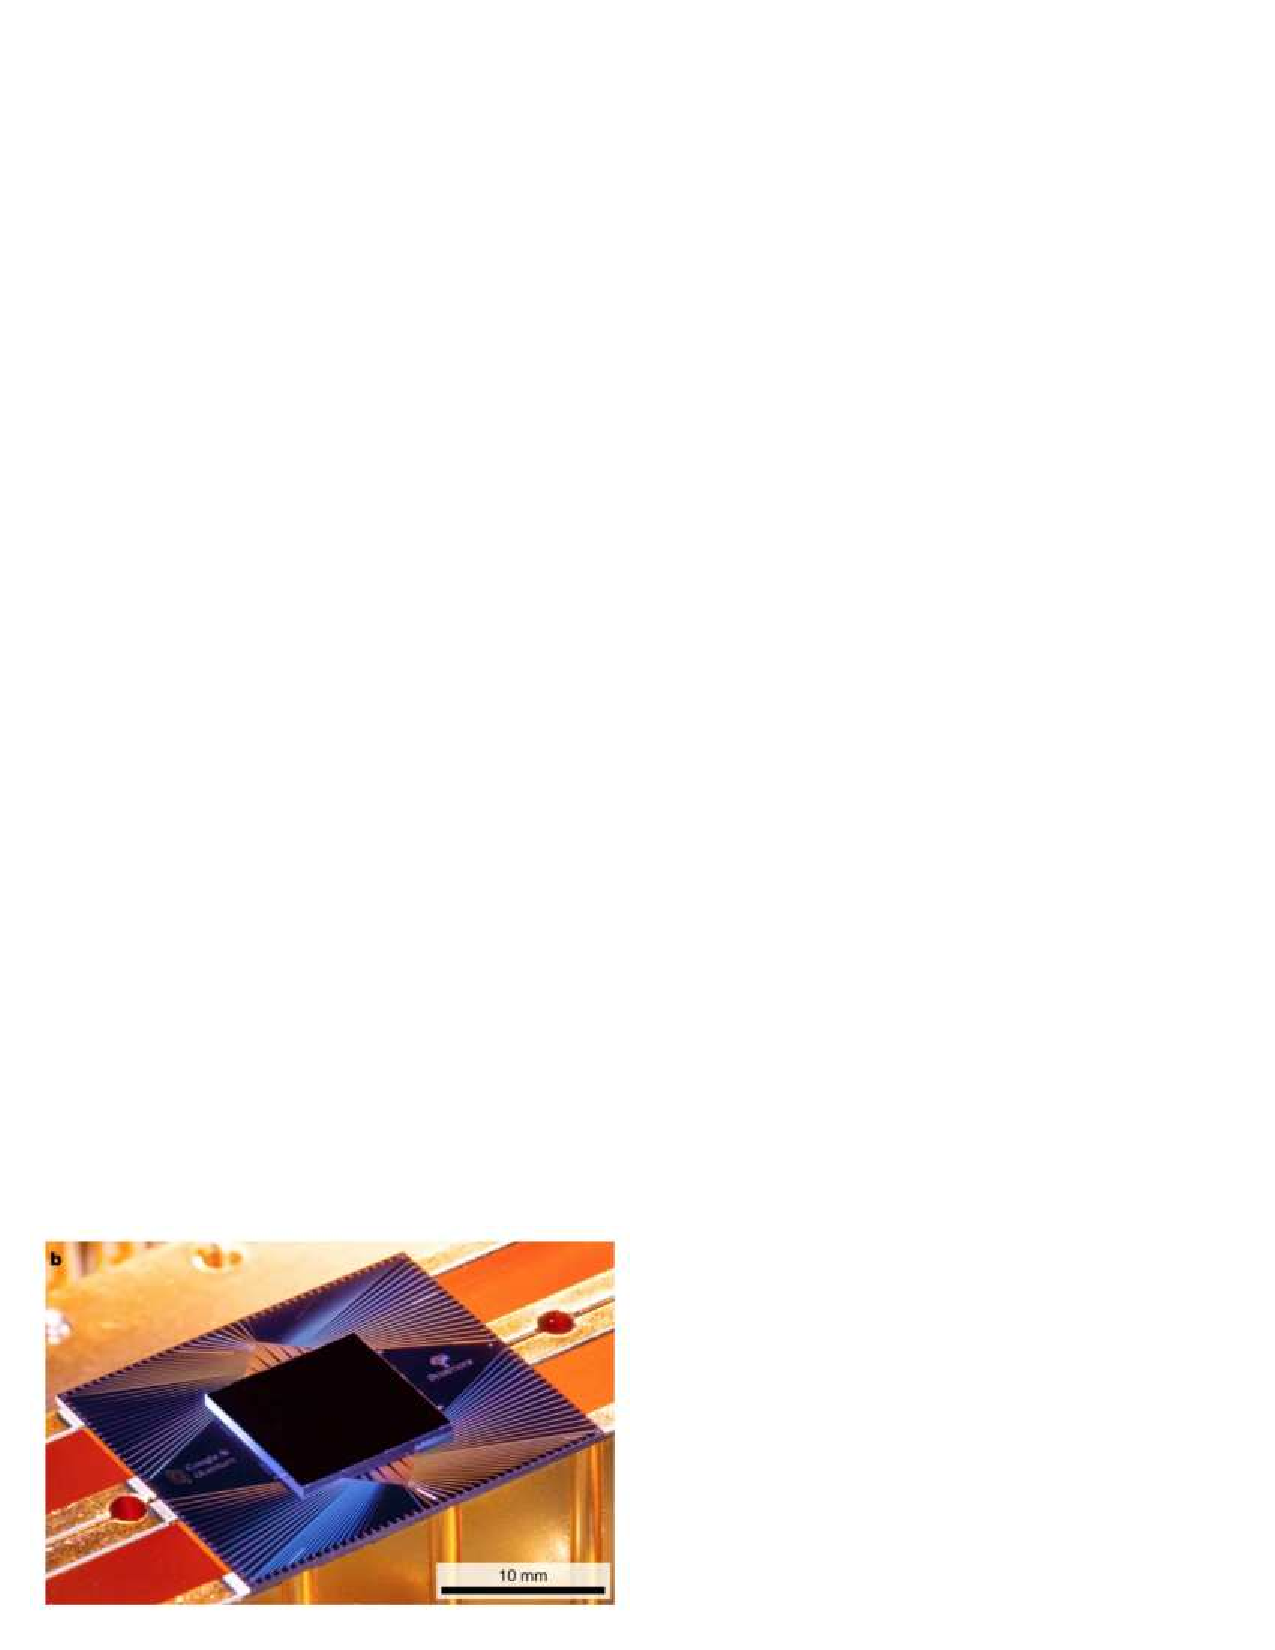
\includegraphics[scale=0.8]{img/sycamore.pdf}
  \caption{Photograph of the Sycamore chip.}
  \label{fig:sycamore_processor}
\end{figure}

...

...

...

%%%%%%%%%%%%%%%%%%%%%%%%%%%%%%%%%%%%%%%%%%%%%%%%%%%%%%%%%%%%%%%%%%%%%%%%%%%%%%%%%%%%%%%%%%%%%%%%%
%
% The following paragraph contains an example of a bullet list. Use the
% environment \begin{itemize} ... \end{itemize} to produce an itemized/bullet
% list. Each bullet is defined with the command \item 
%
%%%%%%%%%%%%%%%%%%%%%%%%%%%%%%%%%%%%%%%%%%%%%%%%%%%%%%%%%%%%%%%%%%%%%%%%%%%%%%%%%%%%%%%%%%%%%%%%%
The qubit is encoded as the two lowest quantum eigenstates of the resonant
circuit. Each transmon has two controls:

\begin{itemize}
  \item  A microwave drive to excite the qubit, and
  \item A magnetic flux control to tune the frequency.
\end{itemize}

Each qubit is connected to a linear resonator ...

...
\graphicspath{ {./images/} }

\section{Experiments}
\label{sec:experiments}

\subsection{State machines}
I wanted to create something where you could enter a state, invoke the start function once, and then repeatedly invoke the update function. I tried to do this with structs, but I couldn't get it to work. I ended up using a switch statement to check the state and then execute the corresponding code. I am not sure if this is the best way to tackle this, but it sure is a way that I think works pretty okay and is easily understandable.

\subsection{Interrupts}
I had never worked with interrupts before in embedded systems, so I had to do some research on how to use them. I found a good tutorial that explained how to use them. I used the same method for both the horn and the brake. Eventually, I also got word that I had to use interrupts for the Hall sensor, but sadly I didn't get this to work. I hope to eventually look into the Hall sensor again since it is a useful component.

\subsection{Hall sensor}
I have tried to get the Hall sensor working, but I was not able to get it working. I have tried multiple different ways to get it working, for example:
\begin{itemize}
    \item Interrupts
    \item While loops
    \item GPIO readings
\end{itemize}
Sometimes I ended up with a value between 0-10 which spiked to more than 1000, or I ended up with backtrace errors. Eventually, I just wanted to be done with it so I decided to leave it out for now.

\subsection{Motor}
I was struggling a lot with my motor. All the documentation I could find was for Arduino. Not everywhere did it mention the need for an external power source, and when I thought I had it right, not much happened. I went through three DC motors because they stopped working. I tried to repair one, but unfortunately, it didn't yield any results. 
\\ \\
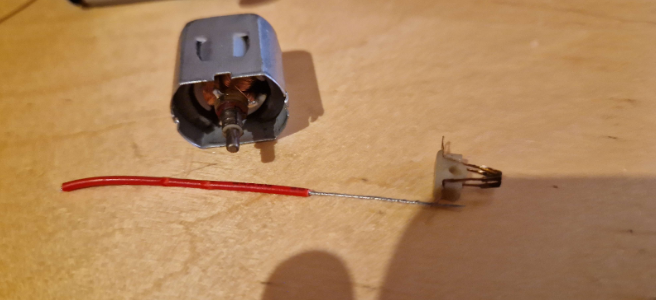
\includegraphics[scale=0.5]{img/motor.png}
\\ \\
Finally, I managed to get the motor running once and adjust the speed with the potentiometer. However, it only worked in one direction because as soon as I connected \texttt{MOTOR\_IN2\_PIN} correctly, it stopped, seemingly due to the current coming out of the driver. I tried to use a multimeter to figure out where it started or what caused it, but I couldn't get any clearer information. So I just hard coded it to the ground as a quick fix.
\\ \\ 
\href{https://drive.google.com/file/d/1rd44Cz8T1Gg5iTYCPDCrZmAVjVKYmPvb/view?usp=sharing}{\textbf{em2-motor-test1.mp4}}
\\ \\ 
I was still super happy that at least it worked in one direction, but when I tried to start it again the next day, it didn't work anymore. And just like how it suddenly didn't work again, it suddenly started working again. I have no idea what caused it to stop working or what caused it to start working again. I'm just happy it works now.
\\ \\ 
\href{https://drive.google.com/file/d/1BRR4opuRYfXWmIPmIqXvLAS7DdbljeMK/view?usp=sharing}{\textbf{em2-motor-both-sides.mp4}}
\\ \\ 

\section{Conclusions}
\label{sec:conclusions}
Quantum processors based on superconducting qubits can now perform computations
in a Hilbert space of dimension $2^{53} \approx 9 \times 10^{15}$, beyond the
reach of the fastest classical supercomputers available today. To our knowledge,
this experiment marks ... 
%
%%%%%%%%%%%%%%%%%%%%%%%%%%%%%%%%%%%%%%%%%%%%%%%%%%%%%%%%%%%%%%%%%%%%%%%%%%%%%%%%%%%%%%%%%%%%%%%%%


%%%%%%%%%%%%%%%%%%%%%%%%%%%%%%%%%%%%%%%%%%%%%%%%%%%%%%%%%%%%%%%%%%%%%%%%%%%%%%%%%%%%%%%%%%%%%%%%%
%
% Bibliography
%
% This command will print the references/bibliography at the end of your research paper.
%
\printbibliography[heading=bibintoc]
%
%%%%%%%%%%%%%%%%%%%%%%%%%%%%%%%%%%%%%%%%%%%%%%%%%%%%%%%%%%%%%%%%%%%%%%%%%%%%%%%%%%%%%%%%%%%%%%%%%


\end{document}          % End of your research paper.
